\chapter{Computational models of analogical reasoning}
\label{chapter:1}


\initial{I}n this first chapter, we provide an overview of various attempt to
formalize and theorize analogical reasoning, with a strong emphasis on
computational models. We will be led at the end of this chapter to the so
called Boolean analogical proportions and their use in machine learning, which
were the starting point of our research.

\section{Models without proportions}
\label{sec:models_without_proportions}

In his famous book \textit{How to Solve It} \cite{Pol45}, the mathematician
George P\'olya suggests to his readers different ways of reaching the solution
of (mostly) mathematical problems. Among the different heuristics that are
proposed, the analogy has a prominent place. Considering the problem of finding
the center of gravity of a homogeneous tetrahedron, P\'olya suggests to observe
that the tetrahedron and the triangle have many similar features, and to first
find the center of gravity of the triangle: a somewhat simpler problem.

\begin{quote}
Knowing that the triangle and the tetrahedron are alike in many respects, we
  conjecture that they are alike in one more respect. It would be foolish to
  regard the plausibility of such conjectures as certainty, but it would just
  as foolish, or even more foolish, to disregard such plausible conjectures.
\end{quote}

As the center of gravity of a triangle is the meeting point of the three
medians, the analogical argument suggest that the center of gravity of the
tetrahedron is the meeting point of the six median planes. The work of P\'olya
is probably the first occurence of analogical reasoning mentioned as a tool for
problem solving in the modern era.

\subsection{Analogy as a structural mapping}

The role of a structural mapping between a source domain and a target domain
has been recognized for a long time as a key component of analogical reasoning
\todo{ref Polya Vol II}. As such, this principle has led to numerous theories
and computational models that we briefly (and non-exhaustively) recall here.

\paragraph{Gentner's Structure Mapping Theory\\}

Probably the most influential model of analogical reasoning is the Structure
Mapping Theory (SMT), introduced by the American cognitive scientist Dedre
Gentne in \cite{Gen83}. The main feature of SMT is to consider that good
analogies are those that result from strong, deep, relations and dependencies
between the source and the target domains, rather than on some superficial
characteristics. In this regard, SMT departs from Hesse's theory in a
significant way. \todo{mettre ça dans Hesse si Hesse après}

The point of Gentner is that superificial similarities are often irrelevent,
while what matters in an analogy are the underlying \textbf{structural}, high
order relations between the objects at play. To examplify, Gentner argues that
when one says that \textit{a battery is like a reservoir}, the analogy stands
because at some abstract level, a battery and a reservoir serve the same
purpose: to release some potential energy that has been stored for some time.
The fact that batteries come in different shapes, colors and sizes than
reservoirs does not play any role in the relevence of the analogy. This
principle is called the \textbf{systematicity principle}, for which we now give
some technical details.

The world is assumed to be represented by objects (belonging either to the
source domain $S$ or the target domain $T$), along with some
\textbf{predicates} that deal with one or more objects of the same domain. The
distinction is made between predicates that only take one argument
(\textbf{attributes} of objects), and those  that take at least two objects
(\textbf{relations}). Higher-order relations are relations for which arguments
are themselves relations, instead of simple objects. To illustrate these
syntactic distinctions, \textit{TALL(Bob)} and \textit{BLONDE(Alice)} are
attributes over the objects \textit{Bob} and \textit{Alice}.
\textit{ARE\_FRIENDS(Bob, Alice)} and \textit{HAVE\_DINNER(Bob, Alice)} are
first-order relations, and \textit{CAUSE[ARE\_FRIENDS(Bob, Alice),
HAVE\_DINNER(Bob, Alice)]} is a second-order relation.

In SMT, an analogy is defined as a one-to-one mapping $M$ from $S$ to $T$ that maps
relations (and only relations) between the two domains. The systematicity
principle mentioned earlier states that during the mapping, attributes of
objects (considered to be superficial features) are discarded and not taken
into account, while higher-order relations are given priority over lower-order
ones. Also, out of two relations of the same order, the one that is the most
involved into other (higher-order) relations is the most likely to be mapped in
the target domain. This last requirement gives an implicit rule to somehow
assess the relevence of a relation in an analogy.

Note that this definition of analogy involves purely structural and syntactical
features. The semantic underlying the relations (or the objects) are competely
out of concern. In our example, the fact that \textit{Alice} and \textit{Bob}
are actually friends is of no importance: for SMT this relation is nothing but
a first-order relation, with no particular meaning. As far as SMT is concerned,
\textit{Alice} and \textit{Bob} could just as well be arch-enemies, it would
not make any difference during a potential mapping process with a target domain
(which would, for example, involve two other individuals with a similar
relationship).

While SMT is a purely theoretical framework for analogy, these ideas have been
practically implemented in a software called the Structure Mapping Engine (SME)
\cite{FalForKenGen89} written in LISP, leading to numerous
applications.\todo{Lovett?} The SME algorithm, in complete accordance with SMT,
can be conceptually summarized as follows:
\begin{enumerate}
    \item Look for all potential matches between relations in the source domain
      and the target domain.
    \item Try to group matches into maximally consistent collections of
      matches.
    \item From each collections, infer some relations that might stand in the
      target domain.
\end{enumerate}
In its most simple form, the SME algorithm can be viewed as the finding of a
maximum common subgraph between two graphs, namely those reprensenting the
source and the target domains. In such, SME is part of the connectionist
approaches.

In  \cite{ChaFreHof92}, authors point out various concerns about SMT and SME.
Among them is the fact SME is too reliant on the (human-made) description
inputs of the source and target domains, and that the intelligence mostly comes
from these descriptions:

\begin{quote}
  when the program’s discovery of the correspondences between the two situations
  is a direct result of its being explicitly given the appropriate structures
  to work with, its victory in finding the analogy becomes somewhat hollow.
  Since the representations are tailored (perhaps unconsciously) to the problem
  at hand, it is hardly surprising that the correct structural correspondences
  are not difficult to find.
\end{quote}

Also, while the systematicity principle is undoubtly at the core of many
analogies, it should seem natural to challenge it in some other situations. It
is indeed quite easy to find analogies were superficial features are the most
decisive ones \cite{Bar10}.

\paragraph{The Constraint Satisfaction Theory\\}

As one of the most influential theories of analogical reasoning, SMT has opened
the way to various other models such as that of Holyoak and Thagard
\cite{HolTha89}. Here as well, an analogy is considered to be a mapping between
two domains $S$ and $T$\footnote{with the exception that the mapping goes here
from $T$ to $S$.}. Taking over Gentner's systematicity principle (in a relaxed
form), Holyoak and Thagard exhibit two additional dimensions of importance in
an analogical process. First, the semantics behind the objects at hand, i.e.
the meaning that human agents associate with these objects, are taken into
account. In this theory, the two realtions \textit{ARE\_FRIENDS} and
\textit{ARE\_ENEMIES} are not the same. This clearly stands in contrast with
SMT, where all object attributes are simply discarded (along with their
meanings)\todo{Et va dans le sens de Hesse}. Second, this theory also involves
the pragmatic considerations of the human agent: the goal and purpose of the
analogist should somehow guide the mapping process in some direction or
another. Mappings that serve the purpose of the agent are therefore given
higher priority than others.

Another main difference with SMT, where the systematicity principle is a fixed,
inflexible rule, is that here the three dimensions (systematicity, semantic
similarity and pragmaticity) are interpreted as \textbf{constraints} and not as
rigid directions. These constraints are only here to guide the mapping process.

Holyoak and Thagard's theory has been implemented in a LISP software called
ACME (Analogical Constraint Mapping Engine), in a similar fashion as the
COPYCAT program in that they are both cooperative algorithms.\todo{ref a
copycat}. Much like SME, ACME is part of the connectionist approaches.

\paragraph{Heuristic-Driven Theory Projection\\}

Another framework where structural mapping is considered the core of an
analogical process is the so-called Heuristic-Driven Theory Projection proposed
by Gust, K\"uhnberger and Schmid \cite{GusKunSchTCS06}. While in SME and ACME
the main algorithm boils down to finding a maximum common subgraph between the
two domain representations, HDTP banks on a more formal approach. The two
domains are formally described in first-order logic as a set of facts
(variable-less formulas such as \textit{TALL(Bob)}) and a set of laws
(quantified formulas, such as \textit{$\exists x,$ TALL($x$)}). Using an
anti-unification (generalization) process, the two domains (or theories) $S$
and $T$ are mapped through a generalized theory $G$ described in a second-order
logic. As expected from the name of the framework, the way the mapping is
performed is heuristic-based. From this generalized theory, a transfer of
knowledge can be applied to the target domain, thus allowing the inference of
new facts and laws, provided that they are in accordance with the already known
formulas.  This process of generalization followed by a transfer phase is what
is called a \textbf{theory projection}.

\subsection{Something}

\paragraph{A determination rule for analogical inference\\}

We have seen so far many models of analogical reasoning that mostly rely on
some heuristic, intangible principles. In constrast with this tendency, Davies
and Russel proposed a set of conditions required in first order logic for the
analogical inference process to be sound. Concretly, they provide some
sufficient conditions that must hold on two properties $P$ and $Q$ for the
following inference to be sound
$$\infer{Q(T)}{P(S) \wedge Q(S) & P(T)},$$
where $S$ and $T$ are the source and target objects. Naturally, this framework
can perfectly be generalized with many properties $P_1, P_2, \cdots P_n$.

A first obvious option would be to add as a premice the following implication:
$$\forall x, P(x) \implies Q(x).$$
But this is unsatisfactory, because in this case the inference simply reduces
to
$$\infer{Q(T)}{P(T) & \forall x, P(x) \implies Q(x)},$$ where no use of the
source $S$ is made. It is clear that this inference can not be reasonably
considered as an analogy: the additional premise must not lead to a conclusion
by only involving the target $T$. Some knowledge about the source $S$ must be
taken into account.

To solve this issue, Davies and Russel introduce what they call the
\textbf{determination rule} i.e. the fact that the value of $P$ determines that
of $Q$:
$$\left(\forall x ~ P(x) \implies Q(x)\right) \vee \left(\forall x ~ P(x) \implies
\neg Q(x)\right).$$
This reads as \textit{all $P$'s are $Q$'s, or none of them are}. More
generally, this relation can be considered as being a functional dependency
between $P$ and $Q$, i.e. $Q = f(P)$. This determination rule has the two
required properties: it allows a sound deduction of $Q(T)$, and forces to
inspect the source $S$ to rule out one of the two parts of the
conjunction.\textcolor{red}{HOW??? PAS COMPRIS NEED HELP}.



\section{Models with proportions}

\paragraph{The model of Rumelhart and Abrahamson\\}

At a time where most models of analogy take the form of complex computer
programs (such as that of Evans detailed in Section \todo{La ref}), the two
cognitive scientists David Rumelhart and Adele Abrahamsen proposed a simple
theoretical model of analogical reasoning \cite{RumAbr73}. Their model is of
great interest for us because as it will become clear, their view of analogy is
in total accordance with our use of analogy in machine learning (or should we
say more humbly that our use of analogy is fully complient with their earlier
model).

\textcolor{red}{On va parler de proportions et de resolution, est ce que ca a
deja ete mentione avant?}

For Rumelhart and Abrahamsen, a human reasoning process can be defined by two
components: a memory structure in which the remembered objects are stored, and
an algorithm that manipulates these data to produce a result. In their paper,
they define these two components for the analogical reasoning.

With regards to the memory structure, their assumption is that it can be
considered as an $m$-dimensional Euclidean space. This assumption is originally
that of Henley \cite{Hen69} who showed, with the help of social experiments,
that a set of 30 mammals could be fairly well represented in a 3-dimensional
space with axes ferocity, humaness, and size. It is supposed that the semantic
similarity that people associate with two concepts is inveresly proportional to
their distance in the Euclidean space.

Rumelhart and Abrahamsen are interested in the problem of solving an anlogical
equation (although they never state it in these terms): given three concepts
$A, B, C$ and a set of solutions $D_1, D_2, \cdots, D_n$, which $D_i$ is the
best candidate for $A:B::C:D_i$? Their assumption is the following: \textbf{
for a human agent, the best solution is the closest $D_i$ to the (potentially
hypothetical) \textit{perfect} solution $I$, defined as $I = C - A + B$}. This
principle is illustrated in figure \ref{FIG:rumelhart_model}. Diverse social
experiments are led by the authors to assess the soundness of this hypothesis.

\begin{figure}[!h]
\centering
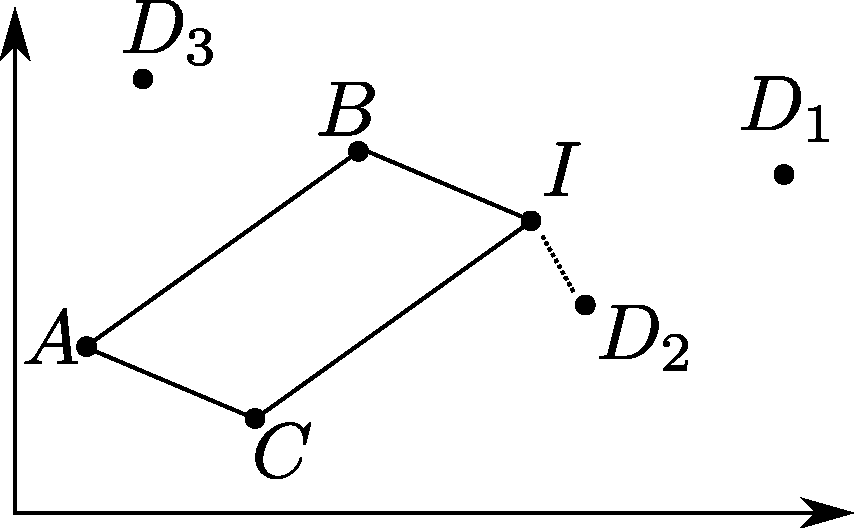
\includegraphics[width=2.5in]{figures/rumelhart_model.pdf}
  \caption{Analogical equation solving process as in \cite{RumAbr73}. The
  solution is here $D_2$.}
\label{FIG:rumelhart_model}
\end{figure}

It is clear that this view of the analogical reasoning process is exactly what
is practically implemented in the experiments of \cite{BayMicDelIJCAI07}, and
all the more so in ours.\todo{ref avant après?}

\paragraph{The Copycat program\\}

Copycat \cite{Mit93} (see also \cite{HofMit94}) is another famous program that
performs analogical reasoning tasks, introduced by Melanie Mitchell and Douglas
Hofstadter. The problems considered by Copycat are the solving of analogical
equations in a \textit{microworld} of strings of letters. A typical Copycat
problem looks as follows: $$\mathbf{abc} : \mathbf{abd} :: \mathbf{ijk} : x$$

What should the value of $x$ be? Various answers may be relevent here, such as
$\mathbf{ijd}$ (replace the right-most letter by $\mathbf{d}$), but the most
natural answer probably is $\mathbf{ijl}$: replace the right-most letter by its
successor. How about $\mathbf{zrq}$? Well, not really convincing. The point of
the authors, however, is that \textit{a priori} every single option should be
given equal chances of success.

This principle is strongly reflected in the Copycat program which is
probabilistic in nature: for the same problem, various solutions can be found
depending on the initial condition. For example the  equation $\mathbf{abd} :
\mathbf{abd} :: \mathbf{mrrjjj} : x$ leads to $\mathbf{mrrkkk}$ in 70\% of the
cases (over 1000 experiments), and to $\mathbf{mrjjk}$ 20\% of the time. Other
less plausible solutions make up the remaining 10\%.

At the beginning of the program, each option is equally available.  Then, on
the basis of their validity, some hypotheses are given a stronger chance to
\textit{survive} till the end of the program, while others are discarded.
Conceptually, this process is emerges from the interoperability of three main
components: the workspace, the codelets, and the temperature.

\begin{itemize}
    \item The workspace, is the place where objects and relations live.
      In the workspace, diverse conceptual structures are built-in:
      \textit{successor}, \textit{predecessor}, \textit{left-most},
      \textit{right-most}, \textit{orientation}, etc. When the program starts, none of these
      structures are activated: this will be the role of the codelets.
    \item The codelets, are competing agents trying to explore and build
      perceptual structures and relations between the objects in the workspace.
      Their behaviour depends on the temparature.
    \item The temperature could be also defined as the entropy of the
      system. When relations in the workspace are strong and well established,
      the temperature is low. At the beginning of the program, the temperature
      is the highest, leading to a multitude of codelets being run in every
      single \textit{direction}. This concept of temperature can be viewed as
      the tradeoff between exploration (trying every possible hypothesis) and
      exploitation (the actual use of a well established hypothesis). When the
      temperature goes below a given threshold, the program stops and the
      current hypothesis is outputed.
\end{itemize}

\begin{figure}[!h]
\centering
  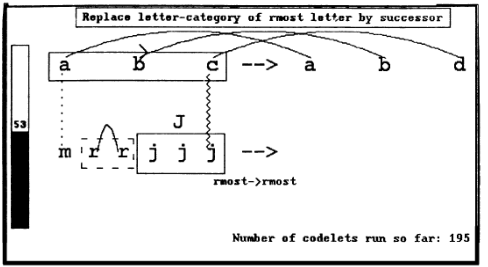
\includegraphics[width=3.5in]{figures/copycat.png}
\caption{Snapshot of Copycat during an equation solving process. Image taken
  from \cite{Mit01}.}
\label{FIG:copycat_snapshot}
\end{figure}

Figure \ref{FIG:copycat_snapshot} illustrate the internal state of Copycat
during the solving of $\mathbf{abc} : \mathbf{abd} :: \mathbf{mrrjjj}: x$. 195
codelets have run so far, so the temperature is average and some structure have
been properly established, such as the \textit{successor group} $\mathbf{abc}$
and the \textit{sameness group} $\mathbf{jjj}$. The $\mathbf{rr}$ group is also
begin defined, though still weaker than the others at this stage. Also, a rule
describing the change from $\mathbf{abc}$ to $\mathbf{abd}$ has been
established: \textit{replace the right-most letter by its successor}. Depending
on the future behaviour of the codelets, this rule with either stick till the
end of the program or change to lead to the most common prediction $x =
\mathbf{kkk}$.

Copycat is clearly a complex adaptative system where a global behaviour emerges
from small, independent parts. According to its authors, \textit{Copycat's
architecture is neither symbolic nor connectionist, nor a hybrid of the two;
rather, the program has a novel type of architecture situated somewhere in
between these extremes}.

\subsection{Analogy and the Minimum Description Length Principle}

Ockham's razor (also Occam), due to the Franciscan philosopher William
of Ockham (1285~-~1347), is a well known principle in machine learning theory.
The main and most useful interpretation of the original latin version states
that when trying to explain a situation, if two hypothesis give the same answer
then the best one is probably the \textbf{simplest} one. In practice, what
makes an hypothesis simple remains quite vague, at least from a computational
point of view. Yet this principle has been formalized into Rissanen's Minimum
Description Length Principle (MDLP) \cite{Ris78}, which is based on Kolmogorov
complexity. Despite the difficulty to build inferential models from this
principle (Kolmogorov complexity is often intractable and impossible to
compute or even to estimate), it has shown to be quite influential in the field
of machine learning, at least from a theoretical point of view.

With this in mind, Antoine Cornuéjols proposed a framework for assessing the
quality of an analogy \cite{CorMLS96} (see also \cite{CorJFA96}). In these
papers, Cornuéjols hypothesizes that the best analogy between a source and a
target model is the one that minimizes its description length, in terms of
Kolmogorov complexity.

Let us first first recall some basic knowledge about Kolmogorov complexity,
before diving into more technical details. The Kolmogorov complexity of a
string of characters $x$, denoted $K(x)$, is the length of the shortest
computer program capable of outputing $x$. $K(x)$ is supposed to capture the
intrinsic complexity of $x$. Intuitively, $K('aaaaabbbbb')$ is supposed to be
lower than $K('abaabbabab')$, because a clear pattern emmerges in the first
string, leading to a simple program: first print $a$ five times, then do the
same for $b$. The second string seems more or less random, which makes it
difficult to factorize into a concize program. In somse sense, the Kolmogorov
complexity captures how well can a string $x$ be \textit{compressed}. The
conditional complexity $K(x \given y)$ is the size of the shortest program that
outputs $x$ when given $y$ as an input.

Now, let's get back to our analogical concerns. As illustrated in figure
\ref{FIG:cornuejols_model}, Cornuéjols considers an analogy as a process
involving an object $x_S$ in a source domain, an object $x_T$ in a target
domain, and two functions $f_S$ and $f_T$ transforming $x_S$ and $x_T$ into
$y_S$ and $y_T$ respectively: $y_S = f_S(x_S)$ and $y_T = f_T(x_T)$. Each
domain $S$ and $T$ \textit{lives} inside a theory or model (namely $M_S$ and
$M_T$), that can describe their corresponding objects.

\begin{figure}[!h]
\centering
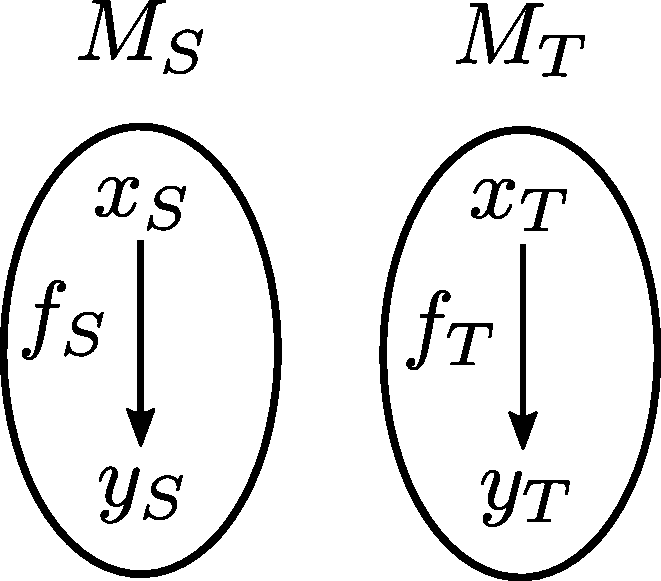
\includegraphics[width=1.5in]{figures/cornuejols_model.pdf}
\caption{The two domains $S$ and $T$ in Cornuejols' model.}
\label{FIG:cornuejols_model}
\end{figure}

For Cornuéjols, the best analogy is the one that minimizes the following sum of
Kolmogorov complexities:
$$K(M_S) + K(x_S \given M_S) + K(f_S \given M_S) + K(M_T \given M_S) + K(x_T
\given M_T) + K(f_T \given M_T),$$
where:
\begin{itemize}
   \item $K(M_S)$ is the cost associated with the source theory,
   \item $K(x_S \given M_S)$ is the cost of $x_S$ as described in the source
     theory,
   \item $K(f_S \given M_S)$ is the cost of $f_S$ as described in the source
     theory,
   \item $K(M_T \given M_S)$ is the cost of describing the target theory from
     the source theory,
   \item $K(x_T \given M_T)$ is the cost of $x_T$ as described in the target
     theory,
   \item and finally $K(f_T \given M_T)$ is the cost of $f_T$ as described in
     the target theory.
\end{itemize}

Notice that the terms $y_i$ are not considered in this cost function, because
they are entirely defined by their corresponding $x_i$ and $f_i$.

Cornuéjols illustrate the plausibility of his model using experiments in the
microworld of Copycat. After defining the Kolmogorov complexity of the built-in
relations (\textit{direction}, \textit{length}, etc.), and those of the
representations of the inputs, the solutions of the analogical equations are
set as those minimizing the above criteria. The empirical results show that
this model, in addition to its theoretical appeal due to the proximity with
MDLP, is at the very least an interesting option to further investigate. In a
recent work , this model of analogy has been applied to a task of transfer
learning \cite{CorMur16}.\todo{Faire lien entre ça et AD de Miclet}

\paragraph{Evans' program to solve geometric problems\\}

The ANALOGY program of Thomas Evans \cite{Eva64} is one of the pioneer work in
the design of programs capable of analogical reasoning. ANALOGY, written in
LISP\footnote{And according to its author, the largest LISP program at the
time!}, is able to solve analogical equations in the form of geometrical
problems, such as that of Figure \ref{FIG:evans}: given three geometrical
patterns, choose the fourth among a list of candidates that leads to the best
proportion.

\begin{figure}[!h]
\centering
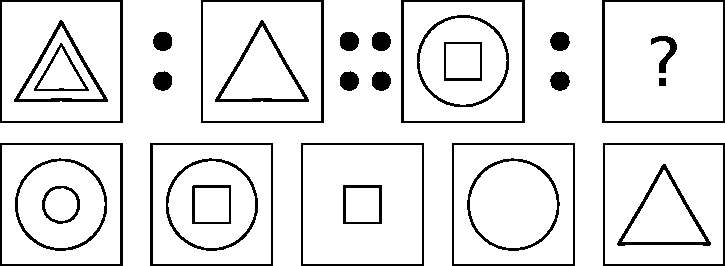
\includegraphics[width=3in]{figures/evans.pdf}
\caption{A geometrical analogy problem}
\label{FIG:evans}
\end{figure}

The inputs to the program are rough, hand-built low-level descriptions of the
figures. For example, simple geometric shape such as circles, rectangles or
triangles are all described with one single primitive:
\textit{SIMPLE\_CLOSED\_CURVE(\dots)}, where the arguments are the start and
end of of the (multiple) lines, and their curvatures. The program is then
devided into two distinct parts.

The role of the first part is to build high level representations of the
figures from these raw descriptions. After identifying coherent shapes (such as
triangle, square, etc) as independent objects, the program tries to find
relations of the kind \textit{INSIDE(Obj1, Obj2)} or \textit{ABOVE(Obj1, Obj3)}
between figures. Finally, similarities between every pair of objects are
computed. The similarity measure is based on the transformability of the first
object into the second one, using tradictional geometrical transformations
(rotation, scale, reflections, etc.). All the information computed by the first
part are given as input (on punched cards!) to the second part.

The second part relates to the analogical solving process per se. Using the
output of the first part, ANALOGY will try to find a set of rules that
transform figure $A$ into figure $B$. A rule would for example state
\textit{REMOVE(Obj1), ROTATE(Obj2, 45\degree), etc.}. Then, by generalizing
each rule, it tries to establish a correspondance between these rules and those
transforming $C$ into one of the candidate solutions. The chosen solution is
that maximizes the resemblance between the two sets of rules.

An interesting fact is that ANALOGY analyses the way to go from $A$ to $B$ and
applies to go from $C$ to $D$, but it does not make use of \textit{central
permutation}: it may just as well analyse the way to go from $A$ to $C$ and
transpose it to go from $B$ to $D$. Note also that in ANALOGY the semantics
behind the relations and the geometrical objects are not taken into account. In
this respect, ANALOGY is close to Gentner's Structure Mapping Theory (and
preexistent by far).

\section{Formal analogical proportions}

An analogical proportion is a statement of the form ``$a$ is to $b$ as $c$ is
to $d$'' involving analogical relations between the pairs $(a,b)$ and $(c,d)$,
as well as between the pairs $(a,c)$ and $(b,d)$.  There are numerous examples
of such statements, with which everybody will more or less agree, such as  ``a
calf is to a cow as a foal is to a mare'', or ``Paris is to France as Berlin is
to Germany''. However, it is only rather recently that formal definitions have
been proposed for analogical proportions in different settings that we briefly
review here.

It has been agreed since Aristotle time that an analogical proportion $A$ is a
quaternary relation satisfying the three following axioms:

\begin{enumerate}
\item $A(a,b,a,b)$ (reflexivity)
\item $A(a,b,c,d) \implies A(c,d,a,b)$ (symmetry)
\item $A(a,b,c,d) \implies A(a,c,b,d)$ (central permutation)
\end{enumerate}

When there is no ambiguity over $A$ and its domain, the infix notation
$a:b::c:d$ is often used.  Considering again our farm example, the symmetry
axiom states that if a calf is to a caw as a foal is to a mare, then a foal is
to a mare as a calf is to a horse, which seems perfectly sound. The central
permutation axiom leads to the natural consequence that a calf is to a foal as
a cow is to a mare.

Starting from the assertion $A(a, b, c, d)$ and by successive application of
the symmetry and central permutation axiom, we arrive to the following eight
equivalent forms:
\begin{align*}
  &A(a, b, c, d)\\
  &A(c, d, a, b)\\
  &A(c, a, d, b)\\
  &A(d, b, c, a)\\
  &A(d, c, b, a)\\
  &A(b, a, d, c)\\
  &A(b, d, a, c)\\
  &A(a, c, b, d)
\end{align*}

Note now that there are exactly $4! = 24$ different orderings of $a, b, c, d$.
We have just seen that $8$ of them form the above equivalence class. There are
two other equivalence classes (each of $8$ orderings, naturally). The first one
is \textit{generated} by $A(a, b, d, c)$ and the second one by $A(a, c, d, b)$.
These theoretical aspects, admittedly tiresome, will however prove useful in
later investigations (Section \ref{Laref}).

There are various models of analogical proportions, depending on the target
domain. We will next review some definitions of analogies in settings that are
of interest for us, but let us first note the following major fact:

\begin{proposition}
  \label{PROPOS:analogy_for_vectors}
  Let $A$ be an analogy over a set $X$. We can define an analogy $A^m$
  over $X^m$ in a component-wise fashion by:
  $$A^m(\mathbf{a}, \mathbf{b}, \mathbf{c}, \mathbf{d}) ~ \emph{  if  } ~
  A(a_i, b_i, c_i, d_i) \emph{ for all } i \in [1, m].$$
\end{proposition}
\noindent
More often than not, $A^m$ will be denoted $A$ for the sake of brevity.

Probably the first use of formal proportions is that of Lepage in
\cite{Lep04} who, starting from the three aforementioned axioms, formally
defined analogical proportions over alphabets of letters with the aim of
generating (analogical) formal languages. His definition have later been
generalized in the works of Stroppa and Yvon (see \cite{StrYvoCNLL05} and
\cite{StrYvoREPORT05})\footnote{In the same work, Stroppa and Yvon also laid
the foundations of analogical learning as used in this thesis (see Section
\ref{la section})}, who provided an algebraic factorization-based definition of
analogical proportions in semigroups:

\begin{definition}
\label{DEF:proportion_semi_group}
Let $(U, \oplus)$ be a semigroup, i.e. $U$ is a set and $\oplus$ is an
  associative binary operation. Four elements $a, b, c, d \in U$, are in proportion if
  there exist some factorization
  \begin{align*}
    a &= a_1 \oplus a_2 \oplus \cdots \oplus a_n\\
    b &= b_1 \oplus b_2 \oplus \cdots \oplus b_n\\
    c &= c_1 \oplus c_2 \oplus \cdots \oplus c_n\\
    d &= d_1 \oplus d_2 \oplus \cdots \oplus d_n,
  \end{align*}

  such that for all $i \in [1, n]$, 
  $$
  \begin{cases}
    a_i = b_i \emph{ and } c_i = d_i\\
    \emph{or}\\
    a_i = c_i \emph{ and } b_i = d_i.
  \end{cases}
  $$
\end{definition}

It will be insighful to instanciate $U$ as the set of natural number
$\mathbb{N}$ and $\oplus$ as the usual multiplication $\times$. In this setting, let's
consider the prime factorization of:

\begin{align*}
  a &= 30 = 1 \times 2 \times 3 \times 5\\
  b &= 60 = 2 \times 2 \times 3 \times 5\\
  c &= 25 = 1 \times 1 \times 5 \times 5\\
  d &= 50 = 2 \times 1 \times 5 \times 5
\end{align*}

For each $i$, we either have $a_i = b_i$ and $c_i = d_i$ ($i = 2, 3, 4$) or
$a_i = c_i$ and $b_i = d_i$ ($i = 1, 4$). We can then say that $a, b, c, d$ are
in proportion, i.e. $30: 60 :: 25:50$. We recognize here the classical
\textbf{geometric proportion}, which states an equality of \textbf{ratios}:
\begin{definition}
\label{DEF:geometric_proportion}
Four real numbers $a, b, c, d$ are in geometric proportion if
$\frac{a}{b} = \frac{c}{d}$, or equivalently if $a\times d = b \times c$.
\end{definition}

It should now be clear for the reader why analogical proportions are
effectively called \textbf{proportions}: it's precisely because they generalize
the well-known numerical (geometric) proportion to other more complex
structures.

Note that the geometric proportion is not the only analogical proportion that
deals with numbers! Indeed, in sections \ref{TODO} we will make use of
the \textbf{arithmetic} proportion, which states an equality of
\textbf{differences}:
\begin{definition}
\label{DEF:arithmetic_proportion}
Four real numbers $a, b, c, d$ are in geometric proportion if $a - b = c - d$.
\end{definition}

Using Proposition \ref{PROPOS:analogy_for_vectors}, four vectors $\mathbf{a},
\mathbf{b}, \mathbf{c}, \mathbf{d}$ of $\mathbb{R}^m$ are in arithmetic
proportion if $\mathbf{a} - \mathbf{b} = \mathbf{c} - \mathbf{d}$, i.e. if they
are the four vertices of a parallelogram, as illustrated in Figure
\ref{FIG:arithmetic_proportion}.

\begin{figure}[!h]
\centering
  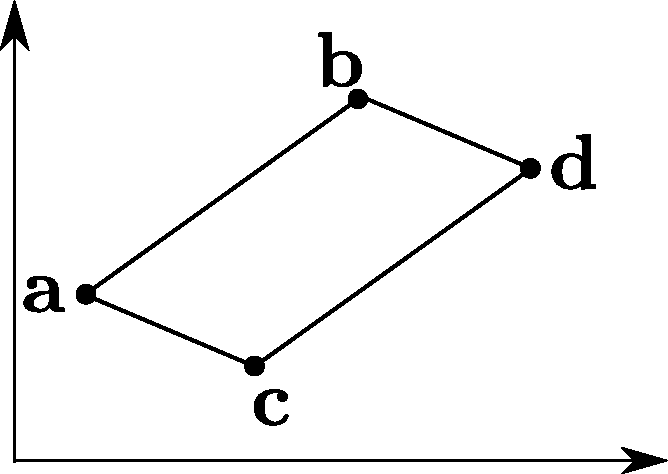
\includegraphics[width=2.5in]{figures/arithmetic_proportion.pdf}
  \caption{$\mathbf{a}, \mathbf{b}, \mathbf{c}, \mathbf{d}$
  are in arithmetic proportion if they are the four vertices of a
  parallelogram.}
\label{FIG:arithmetic_proportion}
\end{figure}

Even if they did not state it in these terms, Rumelhart and Abrahamsen (Section
\ref{TODO}) clearly used the arithmetic proportion for their model of
analogical reasoning.

Beside the use of arithmetic proportion, one of the main focus of this thesis
is to study that of Boolean proportions, i.e.  proportions than one can built
from elements of the set $\mathbb{B} = {0, 1}$. Before diving in more details
into the Boolean proportions, let's first consider the general definition of
analogy in a set, primarly elaborated in \cite{Lep03} as follows: four subsets
$A, B, C, D$ of a universal set $X$ are in proportion if $A$ can be transformed
into $B$ by addind and deleting the same elements as to transform $C$ into $D$.
A more formal definition have been given in \cite{StrYvoREPORT05}:

\begin{definition}
  \label{DEF:analogy_set_facto}
  Let $A, B, C, D \subset X$. $A, B, C, D$ are in proportion if there exists
  four subsets $U, V, W$ and $Z$ (not necessarily disjoint) such that:
  $$
  \begin{cases}
    A = U \cup V\\
    B = U \cup W\\
    C = Z \cup V\\
    D = Z \cup W\\
  \end{cases}
  $$
\end{definition}

To go from $A$ to $B$, one needs to add $W$ and remove $V$. To go from $C$ to
$D$, one needs to do the exact same thing: add $W$ and remove $V$. An
equivalent definition has been given in \cite{MicPra09}:

\begin{definition}
  \label{DEF:analogy_set_miclet_henri}
  Let $A, B, C, D \subset X$. $A, B, C, D$ are in proportion if:
  $$
  A \setminus B = C \setminus D \emph{ and } B \setminus A = D \setminus A
  $$
\end{definition}

Definition \ref{DEF:analogy_set_miclet_henri} reads as \textit{$A$ differs from
$B$ as $C$ differs from $D$, and $B$ differs from $A$ as $D$ differs from $C$},
which is naturally equivalent to the statement of Definition
\ref{DEF:analogy_set_facto}: $A \setminus B = C \setminus D = V$, and $B
\setminus A = D \setminus A  = W$. The formula of Definition
\ref{DEF:analogy_set_miclet_henri} is actually equivalent to the following form
(not without using various ingenious tweaks): $$A \cup D = B \cup C \text{ and
} A \cap D = B \cap C.$$

As an example, let's consider $A = \{a, b, c, g\}, B = \{a, b, d, e, g\}, C =
\{c, f, g\}$ and $D = \{d, e, f, g\}$, as summed-up in Table
\ref{TAB:analogy_sets}.

\begin{table}[h!]
\centering
$$
\begin{tabular}{| c | c  c  c  c  c  c  c |}
\toprule
  & a & b & c & d & e & f & g\\
\midrule
  A & \times & \times & \times &  &  &  & \times \\
  B & \times & \times &  & \times & \times &  & \times\\
  C &  &  & \times &  &  & \times & \times\\
  D &  &  &  & \times & \times & \times & \times\\
\bottomrule
\end{tabular}
$$
\caption{Four sets $A, B, C, D$ in analogical proportion.}
\label{TAB:analogy_sets}
\end{table}

Setting $U = \{a, b, g\}, V = \{c\}, W = \{d, e\}$ and $Z = \{f, g\}$, the
conditions of Definition  \ref{DEF:analogy_set_facto}  are clearly satisfied.
Also, $A \setminus B = C \setminus D = \{c\} = V$, and $B\setminus A = D
\setminus C = \{d, e\} = W$. Finally, $A \cup D = B \cup C = \{a, b, c, d, e,
f, g\}$ and $A\cap D = B\cap C = \{g\}$.

We can also recognize in Table \ref{TAB:analogy_sets} that the conditions of
Definition \ref{DEF:proportion_semi_group} are satisfied, i.e. for all $i$ we
have either $A_i = B_i$ and $C_i = D_i$, or $A_i = C_i$ and $B_i = D_i$. As we
will now see, these two patterns are at the core of the Boolean analogical
proportions, whose definition directly comes from Definition
\ref{DEF:analogy_set_miclet_henri} and by considering the set $\{0, 1\}$:

\begin{definition}
  \label{DEF:boolean_proportion}
  Four elements $a, b, c, d$ in $\mathbb{B} = \{0, 1\}$ are in proportion if
  \begin{alignat*}{2}
    &(a \leftrightarrow b \wedge c \leftrightarrow d) && \vee (a
    \leftrightarrow c \wedge b \leftrightarrow d), \emph{ or equivalently}\\
     & (a \wedge d \leftrightarrow b \wedge c) &&\wedge (a \vee  d
    \leftrightarrow b \vee c),
  \end{alignat*}
  where $\leftrightarrow$ stands for the equivalence connective.
\end{definition}

\todo{Dire qu'il y a plein d'autres modèles, celui la n'est que le minimal}
These scary formulas state the exact same facts as the previous definition,
i.e. that $a$ differs from $b$ as $c$ differs from $d$ and conversely $b$
differs from $a$ as $d$ differs from $c$. Again, an equivalent definition is
that $a, b, c, d$ are in proportion if $a = b$ and $c = d$, or $a = c$ and $b =
d$.

In a Boolean setting, there are exactly $2^4 = 16$ different valuations of $a,
b, c, d$. The only $6$ valuations (or \textbf{patterns}) that lead to a valid
Boolean proportion are illustrated in Table \ref{TAB:six_valid_patterns}.

\begin{table}[t]
  \centering
  $$
  \begin{array}{|cccc|c|}
    \toprule
    a & b & c & d &  A(a, b, c, d)\\
    \midrule
    0 & 0 & 0 & 0 &   \textbf{1}\\
    1 & 1 & 1 & 1 &   \textbf{1}\\
    0 & 0 & 1 & 1 &   \textbf{1}\\
    1 & 1 & 0 & 0 &   \textbf{1}\\
    0 & 1 & 0 & 1 &   \textbf{1}\\
    1 & 0 & 1 & 0 &   \textbf{1}\\
    \bottomrule
  \end{array}
  $$
  \caption{The six valid patterns of the Boolean proportion.}
  \label{TAB:six_valid_patterns}
\end{table}

Table \ref{TAB:six_valid_patterns} provides us with valuable insights. First,
note that some sort of {\it code independence axiom} is satisfied, which
guarantees that $0$ and $1$ play symmetric roles:

\begin{property}
  Let a, b, c, d in $\mathbb{B}$. Then  $a : b :: c : d \iff \neg a :  \neg
  b ::  \neg c :  \neg d.$
\end{property}

Also, it appears that the Boolean proportion is equivalent to the arithmetic
proportion when we restrict it to $\mathbb{B}$:

\begin{property}
  Let a, b, c, d in $\mathbb{B}$. Then  $a : b :: c : d \iff a - b = c - d$.\\
  Note that the geometric proportion offers a necessary condition, but not a
  sufficient one: $a \times d = b\times c$ is satisfied by all of the patterns
  in Table \ref{TAB:six_valid_patterns}, but also for the pattern $0: 0: 0: 1$
  which is not a valid analogy.
\end{property}

Just like in $\mathbb{R}^m$, the arithmetic proportion allows us to think of
Boolean proportions as (potentially \textit{flat}) parallelograms, but this
time we are restricted to $\mathbb{B}^m$. Figure \ref{FIG:proportions_in_B2}
illustrates the proportions that one can build in $\mathbb{B}^2$:
\begin{itemize}
  \item the proportion $\mathbf{a}: \mathbf{b} :: \mathbf{c} : \mathbf{d}$ and
    its 7 other equivalent forms, forming the parallelogram
    $\mathbf{a}\mathbf{b}\mathbf{c}\mathbf{d}$ ;
  \item the proportions that we can build using any pair of vertices, for
    example $\mathbf{a} : \mathbf{d} :: \mathbf{a} : \mathbf{d}$. Each of these
    proportions has three other equivalent forms: in our case $\mathbf{a} :
    \mathbf{a} :: \mathbf{d} : \mathbf{d}$, $\mathbf{d} : \mathbf{a} ::
    \mathbf{d} : \mathbf{a}$ and $\mathbf{d} : \mathbf{d} :: \mathbf{a} :
    \mathbf{a}$ ;
  \item the four proportions involving each vertex independently, for example
    $\mathbf{b}:\mathbf{b}::\mathbf{b}:\mathbf{b}$.
\end{itemize}

\begin{figure}[!h]
\centering
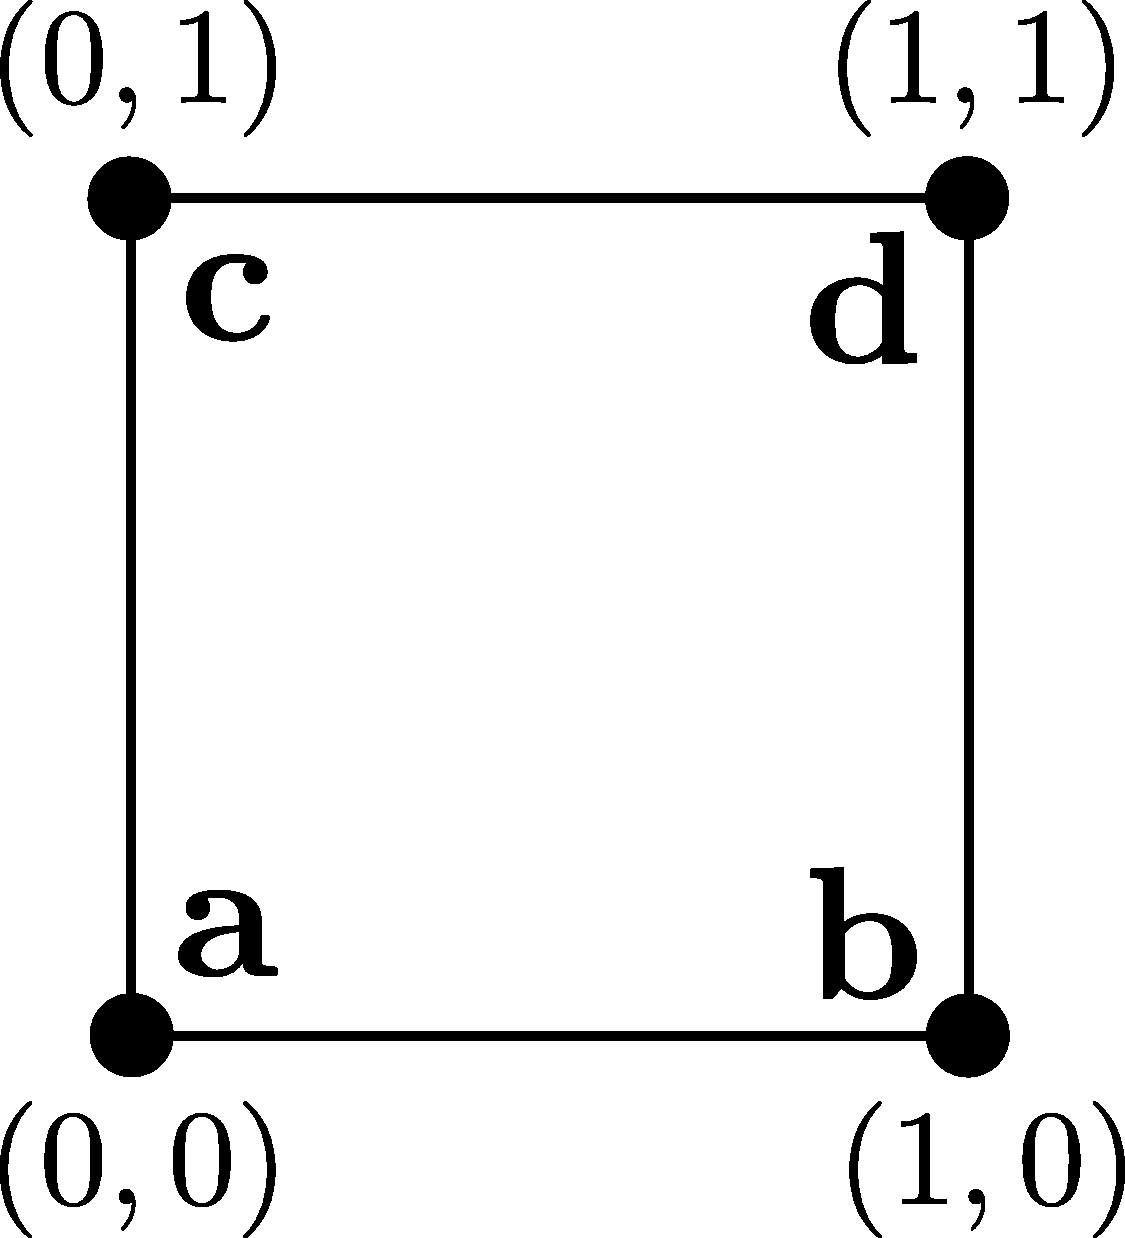
\includegraphics[width=1.5in]{figures/proportions_in_B2.pdf}
  \caption{Proportions in $\mathbb{B}^2$}
\label{FIG:proportions_in_B2}
\end{figure}

All in all, this makes up to $36 = 8 + 6 \times 4 + 4$ proportions, but only $1
+ 6 + 4 = 11$ of them can be considered \textit{unique} (up to equivalence) and
only one is non-flat\footnote{\textit{flat} proportion are those that make up
flat parallelograms. This naming convention is actually fortunate, because
these proportion are in practice absolutely useless.}. In section \ref{TODO},
we will further investigate the number of unique proportions that can be built
in $\mathbb{B}^m$.

Going a dimension further can still be insightful. Figure \ref{FIG:cubes_in_B3}
illustrates the 12 non-flat proportions that exist in $\mathbb{B}^3$. These
proportions are the paralellograms making up the 6 faces of the $3$-cube, and
six other \textit{diagnoal} parallelograms. The flat proportions are not (all)
shown for obvious reasons.

\begin{figure}[!h]
\centering
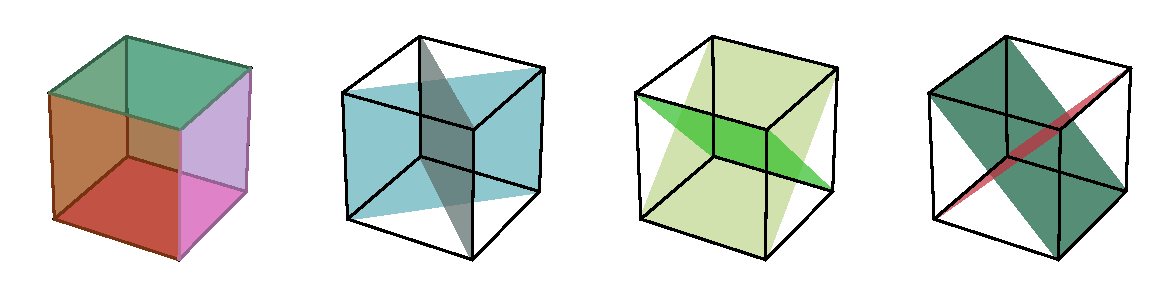
\includegraphics[width=\linewidth]{figures/cubes_in_B3.pdf}
  \caption{The twelve \textit{non-flat} parallelograms in $\mathbb{B}^3$}
\label{FIG:cubes_in_B3}
\end{figure}

\paragraph{Machine learning with Boolean proportions\\}

We now have enough backgroud on Boolean proportions to start doing some machine
learning. Here is our problem. We consider the set $\mathbb{B}^m$ and its $2^m$
elements. For various $\mathbf{x} \in \mathbb{B}^m$, we know the value of
$f(\mathbf{x})$, where $f$ is a function from $\mathbb{B}^m$ to $\mathbb{B}$.
The value $f(\mathbf{x})$ is called the \textbf{class} of $\mathbf{x}$, or its
\textbf{label}. The set $S \subsetneq \mathbb{B}^m$ of elements for which
$f(\mathbf{x})$ is known is called the \textbf{training set}. For any element
$\mathbf{x} \notin S$, $f(\mathbf{x})$ is unknown and our goal is to guess it:
this is a \textbf{classification problem}.

Suppose we're in $\mathbb{B}^3$ and consider Figure
\ref{FIG:classification_problem}.
\begin{figure}[!h]
\centering
  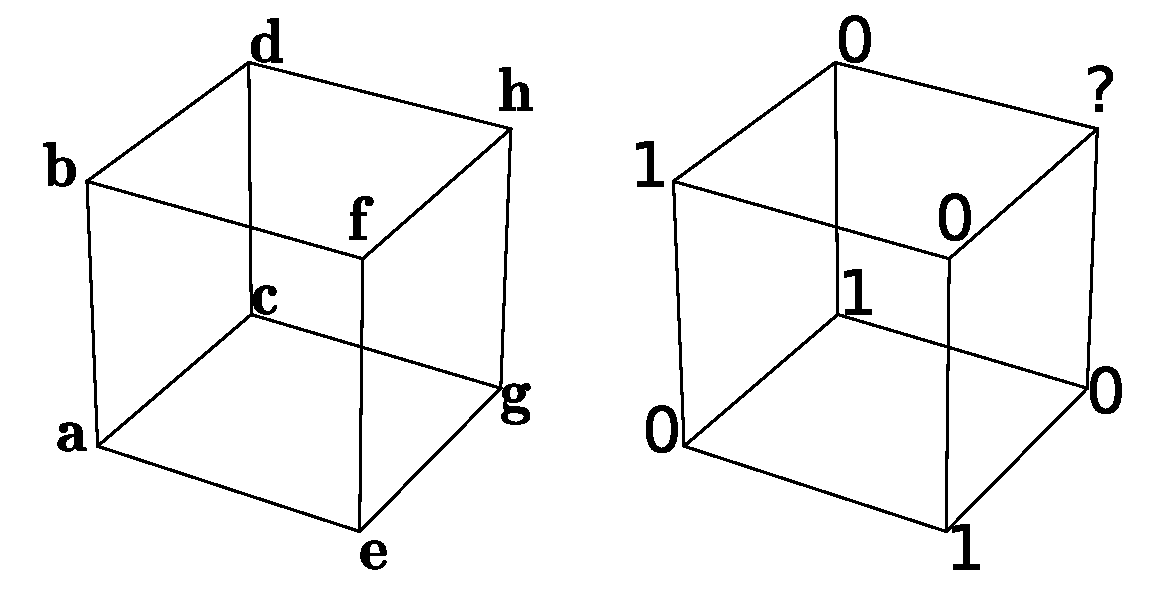
\includegraphics[width=3in]{figures/classification_problem.pdf}
  \caption{What should the value of $f(\mathbf{h})$ be?}
\label{FIG:classification_problem}
\end{figure}
We know the values of $f(\mathbf{x})$ for
every single $\mathbf{x}$ but $\mathbf{h}$, so $S = \{ \mathbf{a}, \mathbf{b},
\mathbf{c}, \mathbf{d}, \mathbf{e}, \mathbf{f}, \mathbf{g}\}$. To guess the value of
$f(\mathbf{h})$, we will use the so-called analogical inference principle,
which states that if four elements $\mathbf{a}, \mathbf{b}, \mathbf{c},
\mathbf{d}$ are in proportion, then their class should also be in proportion:
$$
\infer{f(\mathbf{a}) : f(\mathbf{b}) :: f(\mathbf{c})
: f(\mathbf{d})}{\mathbf{a} : \mathbf{b} :: \mathbf{c} : \mathbf{d}}
$$

This is obviously an unsound principle, in that the conclusion does not
logically follows from the premice. But as we will see in this document, it can
still be useful.

This principle leads us to look for all 3-tuples $(\mathbf{x}, \mathbf{y},
\mathbf{z}) \in S^3$ such that $\mathbf{x}:\mathbf{y}::\mathbf{z}:\mathbf{h}$.
The analogical inference then states that we should have
$f(\mathbf{x}):f(\mathbf{y})::f(\mathbf{z}):f(\mathbf{h})$. Figure
\ref{FIG:cubes_in_B3} tells us that there are 6 (non-flat) parallelograms
involving $\mathbf{h}$ as a vertex. The six corresponding proportions are:

\begin{itemize}
  \item $\mathbf{b} : \mathbf{d} :: \mathbf{f} : \mathbf{h}$
  \item $\mathbf{e} : \mathbf{f} :: \mathbf{g} : \mathbf{h}$
  \item $\mathbf{c} : \mathbf{g} :: \mathbf{d} : \mathbf{h}$
  \item $\mathbf{a} : \mathbf{b} :: \mathbf{g} : \mathbf{h}$
  \item $\mathbf{a} : \mathbf{e} :: \mathbf{d} : \mathbf{h}$
  \item $\mathbf{a} : \mathbf{c} :: \mathbf{f} : \mathbf{h}$
\end{itemize}

Unfortunately, the first three proportion are of no use here. 

Notice that we have light-heartedly ignored  all the flat proportions. This is
because...

\paragraph{How many proportions can we build in $\mathbb{B}^m$?\\}

Exactly $6^m$! And it is fairly easy to derive: there are $6$ proportions in
$\mathbb{B}$. As a proportion in $\mathbb{B}^2$ is the concatenation of any
two propotions in $\mathbb{B}$, there are exactly $6^2 = 36$ proportions in
$\mathbb{B}^2$. Because analogical proportions in $\mathbb{B}^m$ are the
concatenation of $m$ proportions in $\mathbb{B}$ (the proportion is evaluated
component-wise), one can build $6^m$ proportions in $\mathbb{B}^m$.

But let's now ask a more relevent and challenging question: how many
\textit{useful} proportions can we build in $\mathbb{B}^m$? By \textit{useful},
we mean proportions that could be used for classification purposes.

\begin{aquote}{The astute reader, who has been struck by divine light}
  What a silly question! There are obviously $\frac{6^m}{8} - 4^{m - 1} + 2^{m
  - 3}$ such proportions! How can you not be aware of the A016283 sequence from
  the OEIS\footnote{The On-line Encyclopedia of Integer Sequences
  (http://oeis.org/A016283)}?!
\end{aquote}

Unfortunately, we, who have not (yet) been struck by divine light, will have to
derive this formula ourselves. The only proportions
$\mathbf{a} : \mathbf{b} :: \mathbf{c} : \mathbf{d}$ that are useful for
classification purposes are those where all elements $\mathbf{a}, \mathbf{b},
\mathbf{c}, \mathbf{d}$ are distinct.\todo{Expliquer pourquoi selon où on le
met}

We already know that every proportion in $\mathbb{B}^m$ is a parallelogram, and
that there are $6^m$ parallelograms. The geometrical interpretation of the
above statement is that we are here interested only in non-flat parallelgrams,
i.e. parallelograms involving four distinct vertices. We thus want to exclude
from the $6^m$ proportions those that comply with one of the three following
patterns:

\begin{itemize}
  \item $\mathbf{x}: \mathbf{x} :: \mathbf{x} : \mathbf{x}$
  \item $\mathbf{x}: \mathbf{x'} :: \mathbf{x} : \mathbf{x'}$
  \item $\mathbf{x}: \mathbf{x} :: \mathbf{x'} : \mathbf{x'}$
\end{itemize}

Now, let's count them.

\begin{itemize}
  \item Every vertex $\mathbf{a}$ will generate a proportion of the form
    $\mathbf{a}: \mathbf{a} :: \mathbf{a} : \mathbf{a}$, so there are exactly
    $2^m$ proportions $\mathbf{x}: \mathbf{x} :: \mathbf{x} : \mathbf{x}$,.
  \item Every pair $(\mathbf{a}, \mathbf{b})$ of vertices will generate a
    proportion $\mathbf{a}: \mathbf{b} :: \mathbf{a} : \mathbf{b}$, and another
    proportion $\mathbf{b}: \mathbf{a} :: \mathbf{b} : \mathbf{a}$. There are
    $\binom{2^m}{2}$ pairs $(\mathbf{a}, \mathbf{b})$, so in total this makes
    $2\binom{2^m}{2}$ proportions of the form $\mathbf{x}: \mathbf{x'} ::
    \mathbf{x} : \mathbf{x'}$. 
  \item Every pair $(\mathbf{a}, \mathbf{b})$ of vertices will also generate a
    proportion $\mathbf{a}: \mathbf{a} :: \mathbf{b} : \mathbf{b}$, and another
    proportion $\mathbf{b}: \mathbf{b} :: \mathbf{a} : \mathbf{a}$. There are
    thus $2\binom{2^m}{2}$ proportions of the form $\mathbf{x}: \mathbf{x} ::
    \mathbf{x'} : \mathbf{x'}$.
\end{itemize}
